
\section{General Semistructured (Data) Model}\label{def:mofgeneral}
After observing all the definitions provided in the previous sections and chapters, we shall now define a general framework allowing to include all the aforementioned nested representation, including the aggregation requirements provided in the previous sections. We must also consider that any object can nest several objects, and that any object can contain several others simultaneously. 

Contrariwise to other approaches which distinguished atoms (e.g., numbers, strings) from objects (e.g., tuplets, documents, object-oriented objects) and collections \cite{Magnani06}, the proposed \textsc{Generalized Semistructured data Model} provides a uniform representation of the three data representations. This characterisation implies the absence of a binding between a fixed schema and the data representation.

The uniform representation of objects and atoms permits collection supporting both representations uniformly. XML documents are an example of where such situation already happens: in fact, both tags and text nodes may appear as the content of one single tag. This solution is achieved within our data model by representing both objects and values by their reference identifier $o$, and by using their identifier to insert them within such collections. The reference number hides both the associated expressions (list of atoms, $\xi(o)$) and labels (list of strings, $\ell(o)$). Moreover, we decide to represent atoms within the meta-model, so that they can be later on used within transformation functions $\stigma$. Therefore, data can possibly embed both model and meta-model information.

However, all current data models (except from programming languages) do not allow a uniform representation of collections as objects and vice-versa. Given that objects may be represented as a property-value association, where values can be either atoms (as in the relational model and property graphs) or objects, we can assume that each property may be associated to a collection of object identifiers. In particular, our data model chooses to implement object $o$ as multimap associations, which are expressed through a $\phi$ function, allowing to represent an object as a collection of collections. In particular, each collection $l$ represented within an object $o$ can be referenced by using its identifying (and associated) property $p$, such that $\phi(o,p)=l$.


\begin{definition}[General Semistructured (Data) Model]
Given a \textsc{MetaModel}  language $\metamodel$ expressing both constraints and values that can be checked by such constraints and a model $\model$ representable in $\metamodel$ ($\abstr(\model)\subseteq\metamodel$), any \textbf{object}\index{object!for the GSM} $o$ is directly represented by its object identifier $o\in \mathbb{N}$. Such object $o$ shall belong to multiple model types\index{type} $\ell(o)\in\partof{\model}$, and has an associated list of expressions $\xi(o)\in\partof{\metamodel}$ expressing either values or constraints associated to $o$. The attribute-value association embedded in each object $o$ is expressed by the function $\phi$: in particular $\phi(o,p)\in\partof{\nat}$ associates $o$ and an attribute $p$ (represented as an expression $p\in\langg$) to a list of objects. $\varphi(o)$ provides all the objects contained by $o$ for any $p$ and is defined as follows:
\[\varphi(o)\eqdef \bigcup_{p\in\lang}\phi(o,p)\]
Therefore, any object $o$ is identified by its id and is completely described by the functions $\ell$, $\xi$ and $\phi$. Consequently, any instance of the GSM is described by the following quintuple:
\[GSM=(o,O,\ell,\xi,\phi)\]
where $O\subseteq \nat$ is a finite list of object identifiers containing all the elements nested in the \textbf{reference object}\index{object!for the GSM!reference} $o$ at any nesting level ($\varphi^*(o)=O$), thus defining $o$ as multiple collections of objects ($\varphi(o)\subseteq O$). Moreover, the labelling function $\ell$, the expression and data function $\xi$ and the containment function $\phi$ are both defined over $o$ and over each element in $O$. Formally, we have $\ell\colon O\to \partof{\model}$, $\xi\colon O\to \partof{\metamodel}$ and $\phi\colon O\to \metamodel\to\partof{O}$, which are all finite functions.

%We assume that the object with id $0$ is the empty object ($\varphi(0)=[]$, $\xi(0=[]$, $\ell(0)=[]$).
\end{definition}

In particular, we are going to provide the $\metamodel$ language associated to GSMs in Section \vref{sec:scriptEll}. For the moment, we  focus on the data representation aspects of GSM, and later on on the simple queries that can be performed on such model from the integration point of view (Section \vref{subsec:nested-partof}). 

\begin{figure}[!t]
	\centering
	\begin{minipage}{.45\textwidth}
		\centering
		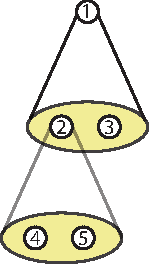
\includegraphics{fig/04model/01SimpleNesting}
		\subcaption{This picture provides a representation of a data structure containing two different nesting levels. Each object is represented by a circle, while
			the containment $\varphi$ function of each object is represented by the cone departing from each object. Within this graphical representation, the leftmost nested object is the first object appearing in the containment function $\varphi$.}
		\label{fig:01simplenesting}
	\end{minipage}\quad \begin{minipage}{.45\textwidth}
		\centering
		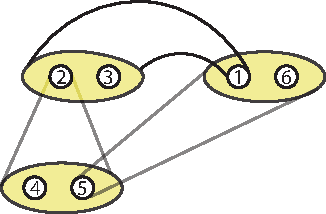
\includegraphics{fig/04model/02RecursiveNesting}
		\subcaption{The data model that is now provided is as general as possible, and hence can support any possible representation. This also implies that recursive nestings are allowed. In particular, this Figure shows that node $2$ may contain elements $4$ and $5$, which contains $6$ and $1$ which contains $1$ back. Therefore, $\varphi(2)=[4,5]$, $\varphi^2(2)=[1,6]=\varphi(5)$, and $\varphi^3(2)=[2,3]$. This recursive nesting solutions should be avoided for representing aggregations.}
		\label{fig:02recursivenesting}
	\end{minipage}%
	\bigskip 
	
	\begin{minipage}{.45\textwidth}
		\centering
		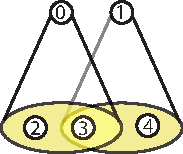
\includegraphics{fig/04model/03Overlapping}
		\subcaption{This picture shows how the $GSM$ model allows to nest one element (e.g. $3$) in more than one single element. In particular, $\phi(0)\cap\phi(1)=[3]$.}
		\label{fig:03overlapping}
	\end{minipage}
	\caption{Different possible instances of the $GSM$ model, allowing arbitrary nestings within its objects. These pictures show some situations that cannot be natively expressed by the current nested relational model and other semistructured representations. In particular, each cone represents one single association between the containing object and its content through an expression $p$.}
\end{figure}
\begin{example}[label=ex:nineteedGSMfrst]
	Figure \vref{fig:01simplenesting} provides an example of a $GSM$. In particular, this model can be modelled as follows:
	\[(1,\Set{1,2,3,4,5},\ell,\xi,\phi)\]
	\[\phi(1,p)=[2,3]\qquad \phi(2,p)=[4,5]\]
	In particular, the containment function maps the object to the contained objects by returning the last ones in a list. This data structure may become
	relevant in some domain specific applications, such as semistructured information, in which the order in which such data appear is relevant. Within our
	examples, we will graphically represent such containment order from left to right. Please also note that ``$o$'' can be arbitrarily chosen from any element in $O$.
	
	Moreover, this data model allows to represent objects as single entities through $\ell$ and $\xi$, and as collections or collection of collections. With respect to the current example, we can consider nodes $3$, $4$ and $5$ with empty nestings as empty collections of objects.
\end{example}

At this point the following question arises: ``\textit{why identifiers} (also referred as ``indices'') \textit{are crucial within nested data structures?}'' As previously discussed, object identifiers also provide a solution to the data replication problem: by only storing the object identifier, we allow that one single piece of information is replicated in more that one single point within the database, thus allowing to overcome some limitations within semistructured data representations.

\begin{example}[continues=ex:nineteedGSMfrst,label=ex:nineteedGSMsnd]
	Figure \vref{fig:03overlapping} represents the following $GSM$ model:
	\[(0,\Set{0,1,2,3,4},\ell\,\xi,\phi)\]
	\[\phi(0,p)=[2,3]\quad \phi(1,p)=[3,4]\]
	In particular, we can see that element $3$ is contained by both $0$ and $1$. This solution is only possible by using explicit identifiers that map objects to its content, typing and value information.
\end{example}

We can use this data model as the most general representation of data structures. Please note that this data model allows arbitrary nestings, such as ``an element can contain itself'' ($\exists o\in O.\exists p\in\lang. o\in \phi(o,p)$) or  ``contain an element that, at any nesting level, contains the container object'' ($\exists o,o'\in O.\exists n\in\nat_{>0}.\exists p,p'\in\lang. o'\in \phi(o,p)\wedge o\in \phi^n(o',p')$). 

\begin{example}[continues=ex:nineteedGSMsnd]
	Figure \vref{fig:02recursivenesting} provides an example of arbitrary nesting levels. In particular, if we choose to use $2$ as the main element within our data model, we can have the following data model:
	\[(2,\Set{1,2,3,4,5,6},\ell,\xi,\phi)\]
	\[\phi(2,p)=[4,5]\quad \phi(5,p)=[1,6]\quad \phi(1,p)=[2,3]\]
	%If we want to refer to all the nestings associated to every $p\in\lang$, we shall refer to the $\varphi$ function which is defined as follows:
	%\[\varphi(o)=\bigcup_{p\in\lang}\phi(o,p)\]  
	If we want to focus on the arbirary nesting levels of node $2$, we shall use the power notation over $\varphi$, where $\varphi^{n+1}$ is recursively defined as the application of $\varphi$ to any element of $\varphi^n$. Therefore, given that $\varphi(4)$, $\varphi(6)$ and $\varphi(3)$ map to the empty set, we can have the following situation:
	\[\varphi(2)=[4,5]\quad \varphi^2(2)=[1,6]\quad \varphi^3(2)=[2,3]\]
	In particular, we are going to refer to any power $n$ as \textbf{(nesting) depth}\GSMindex{depth}. 
	As we can see, this means that $2$ may contain itself at the nesting depth of $3$. Since that this model always allows arbitrary nesting levels, we will use the Kleene plus\index{$\varphi^+$|see{Kleene plus}}\index{Kleene plus} notation, which is defined as follows:
	\[\varphi^+(o)=\bigcup_{n\in\nat_{>0}}\varphi^n(o)\]
	Therefore, we can now express that $2$ contains itself at any level of nesting with the more compact notation $2\in\varphi^+(2)$. Moreover, we can define $\varphi^*(o)$ as the union of $\varphi^+(o)$ with the singleton $\{o\}$ representing the missed application of $\phi$ over $o$ ($\forall x.\varphi^0(x)=\{x\}$).
\end{example}


We can observe that such model features violate the aggregation assumptions presented in Section \vref{sec:informationsintegration}. The reader should remember that aggregations (that can be represented through $\phi$ containments) represent data abstractions:  consequently, neither an object's abstraction can be represented by  the containing object  nor shall the containing object  contain itself at any nesting depth. Since we want that our data model definition can be as slim and as general as possible, we want to express such restrictions as a side properties, similarly to the XML's DTD or RelaxNG. In particular, this thesis is going to focus on a subset of all the possible GSM-based data models (nested graphs included), which are the ones that avoid the recursive nestings presented in the previous example.

\begin{axiom}[Nesting Loop Free]
A general semistructured data model $GSM$ $g\in(o,O,\ell,\xi,\phi)$ is said to be nesting loop free\GSMindex{nesting loop free} if each object $o\in O$ does not contain itself at any nesting level. More formally:
\[\forall o'\in O\cup\Set{o}.\; o'\notin \varphi^+(o')\]
Objects $o\in O$ having empty $\phi$ containments are referred as \textbf{leaves}\GSMindex{leaf}.
\end{axiom}

Moreover, we shall guarantee that the data operations on nesting loop free $GSM$s shall always return nesting loop free $GSM$ results. This axiom also allows to define the hight at which one object is contained by the other without divergences or the possibility of having many possible nesting levels for the same object. Consequently, we can define a ``relative height'' definition, where the containment-container relationship is expressed through the sign. This function will be later used to select which is the highest child, from which start the GSM visiting task, thus allowing to choose which element allows the visit of most of the contained objects with just one step\footnote{For a more practical definition, see line \ref{v3:contentSort} of the code presented in Appendix \vref{appendix:realignments} in OCaml.}. 

\begin{definition}[Heights]\label{def:heights}
Given a nesting loop fee GSM $g=(o,O,\ell,\xi,\phi)$, the \textbf{relative height}\index{height!relative}\index{$rh$|see {height, relative}}\footnote{See line \ref{v3:rh}.} of two objects $o',o''\in O$ is expressed as the function returning $n$ if $o'$ contains $o''$ after maximum\footnote{Please note that, given that the GSM is nesting loop free, it there exists an $n>0$ such that $\varphi^m(o)=\emptyset$ for any $o\in O$ and $m\geq n$.} $n$ applications of $\varphi$ over $o'$ (\ref{rh:containment}), $-n$ if $o'$ is contained by $o''$ after $n$ applications of $\varphi$ over $o''$ (\ref{rh:content}), or zero if the objects are the same or if they are siblings (\ref{rh:same}). For all the other cases (e.g., if they have a common ancestor), the function is undefined.
\begin{numcases}{rh(o',o'')=}
\max S+1 & $S=\Set{n>0|o'' \in \varphi^n(o')},S\neq \emptyset$\label{rh:containment}\\
-(\max S)-1 & $S=\Set{n>0|o'\in\varphi^n(o'')},S\neq \emptyset$ \label{rh:content}\\
0 & $o' = o''\vee \exists o'''\in O.\;o',o''\in\varphi(o''')\wedge o'\neq o'''\wedge o''\neq o'''$\label{rh:same}
\end{numcases}
The former definition can be also used to sort\footnote{See line \ref{v3:contentSort}.} the children $\varphi(o)$ of one single containing object $o$ via their relative height by using the following function\footnote{See line \ref{v3:ho}.}\index{$h_o$}:
\[h_o(o')=\max\Set{rh(o',o'')\neq 0|o''\in\varphi^*(o)\wedge o''\neq o'}\]
Therefore, we can generalize such function to the height of the whole GSM as follows\footnote{See line \ref{v3:h}.}\index{$h$}:
\[h(g)=\max\Set{rh(o,o')\geq 0|o'\in\varphi^*(o)}\]
\end{definition} 

We can also define the concept of ``strongly nested object-set'' by restating the ``strongly connected component'' for graphs over the $\varphi$ containment function. In this case, we want to select from $O$ of a GSM $g$ the sets that contain both the containers and their contents, recursively towards their respective leaves.

\begin{definition}[Strongly nested object-set]\label{def:stronglynestedobjectset}
Given a GSM $g=(o,O,\ell,\xi,\phi)$, it is said that $O'\subseteq O$ is a \textbf{strongly nested object-set}\index{strongly nested!object-set}\GSMindex{strongly nested (object-set)} of $g$ if each object in $O'$ is either a container or a content of another different object of $O'$ ($\forall u,v\in O'. u\neq v'\Rightarrow u\in\varphi^+(v)\vee v\in\varphi^+(u)$). \medskip

We also say that $O'$ is a \textbf{strongly nested object-set component}\index{strongly nested!object-set component} of $g$ if $O'\subseteq O$ and if $O'$ is a maximal strongly nested object-set: this means that it does not exist any object-set $O''$ such that $O'\subset O''\subseteq O$ and $O''$ is a strongly nested object-set. \medskip

If we also fix a subset $\delta O\subseteq O$, then we can also say that $O'$ is a \textbf{strongly nested object-set (component) with respect to $\delta O$}\index{strongly nested!object-set (component) with respect to} if $O'$ is a strongly nested object-set component of $O$ such that $O'\subseteq \delta O$. Therefore, $\delta O$ provides an upper bound for $O'$.
\end{definition}

As a consequence, we have that the desired definition matches with $\varphi^*$. 

Given that the concept of ``subset'' is present both in relational data (via set theory) and on property graphs (via the ``subgraph'' definition from graph theory), we may also provide a similar concept for our GSM model. We're going to use later on this concept for ``filtering'' operators, allowing a partial extraction of the given data structures. We can also use the notion of ``subgraph'' or ``subset-of'' for GSMs and define it as follows:
\begin{definition}[Substructure]
Given two GSMs $g=(o,O,\ell,\xi,\phi)$ and $g'=(o',O',\ell',\xi',\phi')$, it is said that $g'$ is a \textbf{substructure}\GSMindex{substructure} of $g$ ($g'\subseteq g$) if and only if it
 exists a transcoding function $\stigma(o_{c+1})=o_c$, usually called \textbf{morphism} in graph literature, mapping each object in $O'$ to one single object in $O$, where each pair of correspondent objects $o_{c+1}$ and $o_c$ maintain the same labels and expressions, but their containment functions are one the subset of the other:
\[\begin{split}
\forall o\in O'. &\ell'(o) = \ell(\stigma(o))\wedge\\
&\xi'(o) = \xi(\stigma(o))\wedge\\
&\forall p\in\lang. \stigma(\phi'(o,p))\subseteq \phi(\stigma(o),p)\\
\end{split}\]
When the transcoding function is made explicit, we denote the substructure relation as $g'\subseteq_\stigma g$.
\end{definition}

From this basic definition, we can infer the definition of GSM equivalence, where objects' labels, expressions and containments are compared independently from the id appearing in $O$.

\begin{definition}[GSM Equivalence]
	Given two GSMs $g=(o,O,\ell,\xi,\phi)$ and $g'=(o',O',\ell',\xi',\phi')$, it is said that $g'$ abd $g$ are equivalent ($g'\equiv g$) if and only if it
	exists a bijective transcoding function $\stigma$ through which $g'\subseteq_\stigma g$ and $g\subseteq_{\stigma'}g'$.
\end{definition}

\subsection{\texttt{script}, a \textsc{MetaModel} for GSM}\label{sec:scriptEll}
%\section{\texttt{script}}
We now describe the language that we want to express the $\metamodel$\index{\texttt{script}} for our GSM model; \texttt{script}\footnote{See \url{https://bitbucket.org/unibogb/gsql-script/src/f903ff35f16ce2ec6b64bf3a87d68e84e14897e8/src/main/java/it/giacomobergami/nestedmodel2/model/languages/script/?at=master} for the source code implementing such language. Within this project, you can see the actual implementation of some functions that will follow, such as $toNumeric$, $toFunction$ $toList$ that are going to be used within the following denotational semantics.} is an untyped imperative language with dynamic scope and shallow binding, where each program is represented by a list of expressions which are lazy evaluated. Each program returns the value  resulting from the evaluation of the last statement. The \texttt{script} syntax is depicted in Listing \vref{def:script}: \texttt{script} provides some native operations over numbers (either bignum integers or doubles, $\mathbb{Z}\cup\mathbb{Q}$), strings, booleans and lists. All those types are considered compatible between each others, that is they always allow a conversion into a specific representation. Therefore, this language aims to define transcoding functions that can be used for object transformations.



\begin{lstfloat}[!p]
\begin{lstlisting}[language=antlr,caption=Subset of the \texttt{script} language in Antlr4.,label=def:script,basicstyle=\ttfamily\footnotesize]
script  : (expr ';')* expr ;

expr : '(' expr ')'                    #paren
| expr '+' expr                        #number add
| expr '-' expr                        #number subtract
| expr '/' expr                        #number divide
| expr '*' expr                        #number multiply
| expr '++' expr                       #string concatenation
| expr '@' expr                        #list append
| expr '&&' expr                       #boolean and
| expr '||' expr                       #boolean or
| 'not' expr                           #boolean negation
| expr '=='    expr                    #equals
| expr '!='    expr                    #not equals
| expr '<='    expr                    #less equal
| expr '>='    expr                    #greater equal
| expr '>'     expr                    #greater
| expr '<'     expr                    #less
| expr ':='    expr                    #assignment
| expr '.'     expr                    #method invocation
| '(' expr  expr ')'                   #apply right element to left function
| expr '=>' expr                       #if left is true when bool evaluated, 
                                       # return it, otherwise return right
| 'if' expr 'then' expr 'else' expr    #if ... then ... else
| 'substring(' expr ',' expr ',' expr ')' #substring (or sublist of first, 
                                       #between the second and third index)
| expr '[' expr ']'                    #get the element indexed with right in left
| expr '[' expr ']:=' expr             #put the rightmost expression
| expr 'in' expr                       #contains
| 'remove' expr 'from' expr            #remove left element from right list
| EscapedString                        #native string
| BOOL                                 #native boolean
| NUMBER                               #native number
| '{' (expr ',')* expr '}'             #native expressions' array
| VARIABLE '->' '{' (expr ';')* expr '}'#lambda function
| VARIABLE                             #variable
| 'map(' expr ':' expr ')'             #map left list over right function
| 'select(' expr ':' expr ')'          #select left elements using right pred.
;

BOOL : 'tt' | 'ff' ;
VARIABLE   : [a-z]+ ;
EscapedString : '"' ( '""' | ~["\r\n] )* '"';
NUMBER : [0-9]+ (','[0-9]+)? ;
\end{lstlisting}
\end{lstfloat}

This language adopts the implicit casting while evaluating the native operations. As a consequence, the \texttt{number add} operator \texttt{+} is implemented as a binary function $+$ taking a pair of numbers as an input and returning another number:
\[+\;\colon\;\mathbb{Z}\cup\mathbb{Q}\times \mathbb{Z}\cup\mathbb{Q}\to \mathbb{Z}\cup\mathbb{Q}\]
Consequently, the following expression:
\begin{center}
	\texttt{expr$_1$ + expr$_2$}
\end{center}
will be interpreted\footnote{A complete discussion of \texttt{script}'s denotational semantics \cite{Nielson92} goes beyond the goals of the present thesis. In brief, we use the notation $\jsem{P}_\Gamma$ instead of the less intuitive $\Gamma\jsem{P}$.} as follows:
\[\jsem{\texttt{expr}_1 + \texttt{expr}_2}_\emptyset=\textit{toNumeric}(\jsem{\texttt{expr}_1}_\emptyset)\;+\;\textit{toNumeric}(\jsem{\texttt{expr}_2}_\emptyset)\]
where $\emptyset$ represents the environment $\Gamma$\index{$\Gamma$!\texttt{script}'s environment} with which such expressions are evaluated; this means that for the moment, $\Gamma$ does not influence the outcome of the expression's evaluation. Such implicit casting operations allow to reduce the number of the  data-type specific operations, such as defining the length of the list,that can be expressed as outlined in the following example.
\begin{example}
	We want to evaluate the following \texttt{script} expression:
	\begin{center}
		\texttt{0 + \{1, 2, 3\}}
	\end{center}
	where a bignum \texttt{0} is added to a list\footnote{Please observe that the \texttt{script} notation for a list is \texttt{\{\dots\}}, while the one used for the lists within the GSM model is [\dots]. In this way we can distinguish between the syntactic representation and its semantic one.} \texttt{\{1, 2, 3\}}. Given that our canonical function $toNumeric$ maps each list to its length expressed as bignum integers,
	the following expression will be evaluated to \texttt{3}.
	\[\begin{split}
	\jsem{\texttt{0 + \{1, 2, 3\}}}_\emptyset&=\textit{toNumeric}(\jsem{\texttt{0}}_\emptyset)\;+\;\textit{toNumeric}(\jsem{\texttt{\{1, 2, 3\}}}_\emptyset)\\
	&=\textit{toNumeric}(0)\;+\;\textit{toNumeric}([1,\, 2,\, 3])\\
	&=0+3=3
	\end{split}\]
\end{example}


A similar strategy is used for the definition of the \texttt{map} and filter operator (\texttt{select}). The first operator has the following associated semantics:
\[\jsem{\texttt{map(expr}_1\texttt{ : expr}_2\texttt{)}}_\Gamma=[\textit{toFunction}(\jsem{\texttt{expr}_2}_\Gamma)(x)\mid x\in\textit{toList}(\jsem{\texttt{expr}_1}_\Gamma)]\]
In particular, \textit{toFunction} returns a function if the input is a function itself, or acts as a constant function otherwise. When the first argument is a list, \texttt{map} acts as a mapping function over the list, otherwise if it is a function acts as a concatenation between functions, otherwise if it is a single value, it acts as a function application. Similar considerations can be carried out for \texttt{select}.
%Please note that the fundamental operators are represented as definitions, while all the other the derived operators are provided as examples.

A \texttt{script} program allows to define variables and functions, which declarations creates an association within an environemnt\index{$\Gamma$!\texttt{script}'s environment|textbf}  $\Gamma$. Such environment is a set of variable-expressions associations, that can be updated or defined for the first time with an assignment operation:
\begin{center}
	\texttt{VARIABLE := expr}
\end{center}
Therefore, we have that evaluation of such expression will result into an update of $\Gamma$ as follows:
\[\jsem{\texttt{VARIABLE := expr; c}}_\Gamma=\jsem{\texttt{c}}_{\Gamma\cup \{(\texttt{VARIABLE},\texttt{expr})\}}\]
The \texttt{script} language is also capable of defining recursive functions, through which it is possible to generate numeric sequences, and hence generate enumerations. In particular, the following expression will generate a set containing all the positive natural numbers from $2$ to $5$:
\begin{lstlisting}[language=Script]
f := x -> { if (x >= 5) then x else (x @ (f (x+1)))};
(f 2)
\end{lstlisting}
This language even allows to emulate the result of a fold operation over a set. The following example shows how we can add all the natural numbers from $1$ to $10$ by using the following expression:
\begin{lstlisting}[language=Script]
acc := 0;
sgen := x -> { if (x >= 10) then x else (x @ (sgen (x+1))) };
s := (sgen 1);
select( s : x -> { acc := (x + acc) ; ff } );
acc
\end{lstlisting}
In particular, this program initializes the accumulator \texttt{acc} to zero, defines a set containing all the numbers from $1$ to $10$ and stores it into \texttt{s}, then uses \texttt{select} to iterate over \texttt{s} and produce an empty result while, at each iteration step, \texttt{acc} is incremented by one of the elements contained within \texttt{s}. Last, the result of the accumulation is returned.

Consequently, we can generally define the \texttt{foldl} operator as follows:
\begin{lstlisting}[language=Script]
foldl := x -> {
	acc := x[0];
	select(x[1] : y -> {
		acc := (x[2] {y, acc});
		ff
	});
	acc
}
\end{lstlisting}

Before defining any possible operation over the lists, we must make explicit the meaning of  set operations over lists.

\begin{definition}[Set operations over lists]
	Given a binary set operator $\bowtie$, its definition over lists is defined as follows:
	\[L_1\bowtie L_2 = \texttt{distinct}(L_1\bowtie L_2,=)\]
	where \texttt{distinct} returns the element where the repeated elements are preserved, and only the leftmost instance is kept\footnote{This operator can be also defined in \texttt{script} as:\\ \scriptline{distinct = x -> \{fold [x, y -> \{if (y[0] in y[1]) then y[1] else [y[0]] ++ y[1]\}]\}}}:
\begin{lstlisting}[language=Caml]
let rec distinct l eq =
	let rec removehead x ls =
	match ls with
	| [] -> []
	| h::t -> if (eq h x) then t else h::(removehead x t)
in match l with
| [] -> []
| a::[] -> [a]
| a::b -> a::(removehead a (distinct b))
\end{lstlisting}
\end{definition}

\subsubsection{Using environment $\Gamma$ with external GSM values}\label{label:ucwegsmv}
An interesting feature of such language is its possibility of initializing $\Gamma$\index{$\Gamma$!\texttt{script}'s environment} with external objects prior to the evaluation of the expression: this feature is crucial to manipulate and define predicates over the labels, expressions and containments associated to single objects. For this reason \texttt{script} will reserve variable names ``\texttt{o}'' and ``\texttt{g}'' respectively to the current GSM object of interest represented as an object-oriented \texttt{Object}, and the reference object of the current GSM.
\label{app:JavaObject}
Given a GSM $(o,O,\ell,\xi,\phi)$, we can represent each object $o'\in O$ as an object in a object oriented language. In particular, this\footnote{The following url provides a more complete representation of the code that follows: \url{https://bitbucket.org/unibogb/gsql-script/src/f903ff35f16ce2ec6b64bf3a87d68e84e14897e8/src/main/java/it/giacomobergami/nestedmodel2/model/logical/object/model/object/ObjectModel.java?at=master&fileviewer=file-view-default}.} is the object representation that is used in \texttt{script} for the representation of object as external objects.

\begin{lstlisting}[language=Java,mathescape=true]
class Object {
	id objectId;
	public Object(id i) { objectId = i; }
	
	private List phiFuncs(boolean toObject) {
		List toreturn = new List();
		for ($\lang$ e : $\dom(\phi($objectId$))$) {
			List elist = new List();
			elist.add(e);
			List idlist = new List();
			for (id i : $\phi(id,e)$) {
				idlist.add(toObject ? new Object(i) : i);
			}
			elist.add(idlist);
		}
		return toreturn;
	}
	
	public id   id()       { return objectId; }
	public List ell()      { return $\ell($objectid$)$; }
	public List xi()       { return $\xi($objectId$)$; }
	public List phi()      { return phiFuncs(true); }
	public List phiVisit() { return phiFuncs(false); }
}
\end{lstlisting}

This object will use two different phi implementations: \texttt{phi} can be used to manipulate the containment function, and hence will return the GSM objects as \texttt{id}s, while \texttt{phiVisit} can be used in depth visiting operators for the GSM, and hence will return the GSM objects as \texttt{Object}s. Last, a GSM is represented by its reference object as an \texttt{Object} \texttt{g}. 

\begin{example}
	Suppose to have an object $o = 2345$ within a GSM $(o,O,\ell,\xi,\phi)$, where $o$ is associated to the following values:
	\[\ell(o) = [\mstr{ciao1},\mstr{ciao2},\mstr{ciao3}]\qquad \xi(o) = []\]
	\[\phi(o,\mstr{elemento})=[0,1,2]\qquad
	\phi(o,\mstr{elementu})=[3,4,5]\]
	In particular, we initialize $\Gamma$ by associating ``\texttt{o}'' and ``\texttt{g}'' to the same object $o$. In particular, we can get its id by invoking the \texttt{\textbf{id}} method as follows:
	\[\jsem{\texttt{o.\textbf{id}}}_\Gamma=\jsem{\texttt{o}}_\Gamma.\texttt{\textbf{id}()}=2345\]
	Similarly, finite functions as $\phi(o)$ can be expressed by their graph. Even in this case we can use the method invocation to return the content associated to $\phi(o)$ as a list of lists containing two elements, where the first is an expression $e$ and the second is the content of $\phi(o,e)$.
	\[\jsem{\texttt{o.\textbf{phi}}}_\Gamma=[[\mstr{elemento},\, [0,1,2]],\,[\mstr{elementu},\, [3,4,5]]]\]
	Consequently, from now on we choose to graphically represent the graph of a function\index{function|graph of a,} $f$ as a list of pairs (represented as lists of two elements), where each first element represents an element $x$ from the domain, and the second element represents the values associated to the codomain: if $f(x)$ is a function for some $x\in\dom(f)$, $f(x)$ can be represented in \texttt{script} with the same list representation. This also means that we can easily express the function $\dom$ for functions represneted by their graph as follows:
\begin{lstlisting}[language=Script]
dom := f -> { map(f : x -> {x[0]})}
\end{lstlisting}
	Then, we can use a combination of \texttt{select} and \texttt{get} list accessors to obtain the values $\phi(o,\mstr{elemento})$ by selecting the expected list position:
	\begin{align*}
	&\jsem{\texttt{(select( (o.\textbf{phi}) : x -> \{ x[0] == }\mstr{elemento}\texttt{\}))[0] [1]}}_\Gamma\\
	&= \jsem{\texttt{(select( (o.\textbf{phi}) : x -> \{ x[0] == }\mstr{elemento}\texttt{\}))}}_\Gamma.\texttt{\textbf{get}(0).\textbf{get}(1)}\\
	&= {[x \in \jsem{\texttt{o.\textbf{phi}}}_\Gamma\;|\;{\texttt{x.\textbf{get}(0) == }\mstr{elemento}}\;]}.\texttt{\textbf{get}(0).\textbf{get}(1)}\\
	&= {[x \in [[\mstr{elemento},\, [0,1,2]],\,[\mstr{elementu},\, [3,4,5]]]\;|\;{\texttt{x.\textbf{get}(0) == }\mstr{elemento}}\;]}.\texttt{\textbf{get}(0).\textbf{get}(1)}\\
	&= [[\mstr{elemento},\, [0,1,2]]].\texttt{\textbf{get}(0).\textbf{get}(1)}\\
	&= [\mstr{elemento},\, [0,1,2]].\texttt{\textbf{get}(1)}\\
	&= [0,1,2]\\
	\end{align*}
	In particular, we can use the following shorthand for accessing such values:
\begin{lstlisting}[language=Script,mathescape=true]
e[s] $\eqdef$ (select( e : x -> { x[0] ==  s}))[0] [1]
\end{lstlisting}
	so that we can return the  $\mstr{elemento}$  Consequently, we can write an expression allowing us to map, filter and extend the containment. In particular, the following expression will multiply each id referenced by \mstr{elemento} for $\phi$ by $2$, remove the \mstr{elementu} elements and create a new containment \mstr{neu} containing $1$. The desired expression is the following one:
\begin{lstlisting}[language=Script]
{{"elemento", map( (o.phi) ["elemento"] : x -> { (x * 2) } )}} @ {{"neu", {1}}}
\end{lstlisting}
\end{example}

Last, by using the foldl function previously defined, we can also define $\varphi^+$ within \texttt{script} as follows:
\begin{lstlisting}[language=Script]
varphiplus := x -> {
	(foldl {{}, x.phi, y -> {y[0][1] @ y[1]} })
	@
	(map(x.phi : varphiplus))
}
\end{lstlisting}

Appendix \vref{appendix:realignments} also provides a functional definition of such GSM model through the usage of a functional programming language, OCaml. Moreover, the use case in Section \vref{subsec:nested-partof}. and \vref{subsec:representingisa}. will provide some examples of how such $\Gamma$ environment for GSM values achieves structural aggregations.

\subsection{Characterizing object identifiers}
Before introducing either the operations that are possible on top of this model or the nested graph data model itself, we must consider if we have to provide some further constraints on  object identifiers. In particular, we must assume that each identifier maps to one single and possible data representation.  The same concept was introduced with the Object Identity problem at Section \vref{skolem}, where the Skolem functor $f_\Re$ \index{Skolem functor} always provided an unique mapping between object and its id. Similarly to other presented graph model, we adopted the symmetrical solution, that is the index is mapped to the data and not vice versa. GSM already provides this constraining where containment is defined by the list of object identifiers associated with each object's property.

%This constraint is already provided by the data model itself, where the data is already represented through associations between resource identifiers and values.

An object transformation should always generate a different object with a different id, and shall not update the original object, uniquely referenced with its id, with newly associated values. The reason is twofold: we want that shared nothing distributed algorithms make local changes consistent with the global status of the computation, and that the implementations of GSM over object oriented languages maintain the same object reference over the same already-existing object.  This constraint must be also satisfied by the data operations that manipulate the objects.

In order to do so, we must ask ourselves what is the aim of querying data, and which is a suitable representation of the answer to such query within the data model. If we take SQL as a reference, our final query language must allow the creation of views on top of the main databases (in our case, the $GSM$ itself), without necessarily modifying the underneath data representation to which the result is subjected. The same concept is self evident within the relational algebra: the relations took as an input by the algebraic expression are manipulated within the sequence of operations, and returned as a new relation. Consequently, at each step the data subsumes some changes, either structurally or from the informative content, and new elements are created after each operation. 



Given that the creation of new data within queries implies the creation of new identifiers, it is important that even the data model guarantees the creation of identifiers that are easily referable to a previous computation \cite{bergami2014} for optimiziong some data operations. This feature is going to be curcial for the algorithm that will be used for graph nesting in Chapter \vref{cha:nesting}. In particular, each element $j$ represented at the $i$-th step of computation, should change its id  jointly with its internal representation. In order to do so we're going to use dovetailing functions \cite{odifreddi1992} that associate unique integer numbers to a given pair of numbers:

\begin{definition}[Dovetailing function]
Given a pair of two integers $i,j\in \nat$, the \textbf{dovetailing function}\index{dovetailing function}\index{dovetailing} associates to them an unique integer  $j_i\eqdef dt(i,j)\in\nat$ defined by the following function:
\[j_i\eqdef dt(i,j)=\frac{(i+j)(i+j+1)}{2}+j\]
This can be also showed by the definition of the following \textbf{inverse dovetail function} $dt^{-1}(j_i)$ \cite{bergami2014}:
\[dt^{-1}(j_i)=(dt_{\texttt{Left}}^{-1}(j_i),dt_{\texttt{Right}}^{-1}(j_i))\]
where each single component is defined as follows:
\[dt_{\texttt{Right}}^{-1}(j_i)= j_i - \sfrac{1}{2}\cdot\left(\left\lfloor\sfrac{1}{2}\cdot{\left(\sqrt{8j_i+1}-1\right)}\right\rfloor + 1\right)\cdot \left\lfloor\sfrac{1}{2}\cdot{\left(\sqrt{8j_i+1}-1\right)}\right\rfloor\]
\[dt_{\texttt{Left}}^{-1}(j_i) \eqdef \left\lfloor\sfrac{1}{2}\cdot{\left(\sqrt{8j_i+1}-1\right)}\right\rfloor - dt_{\texttt{Right}}^{-1}(j_i)\]
\end{definition}



In particular, to each element $j$ represented at the $i$-th computational step, the computation shall have an id $dt(i,j)$, and $i=0$ when the object is kept unhalterated from the data representation level. When one of the two numbers has a maximum value (e.g., when the number $L$ of the query operators involved within the computation is known), then we can reduce the size of the generated number as follows:

\begin{definition}[$L$-bounded dovetailing function]
	Given a pair of two integers $i,j\in \nat$ where $i$ is upper bounded by $L$, the \textbf{$L$-bounded dovetailing function}\index{dovetailing function!bounded} associates to them an unique integer  $dt(i,j)\in\nat$ defined by the following function:
	\[dt^L(i,j)=j\cdot(L+1)+i\]
\end{definition}

Such dovetailing function can be also used to uniquely associate a number to a list of numbers. In such contexts we can use the $dtl$ function: 
\begin{equation}\label{eq:dtl}
dtl(l)=\begin{cases}
0 & l = []\\
1+dtr(|l|,dtr(l)) & \textrm{oth.}
\end{cases}
\end{equation}
where $dtr$ is recursively defined as follows:
\[dtr(l)= \begin{cases}
e & l = e::[]\\
dt(h,dtr(t)) & l = h::t\\
\end{cases}\]

This other function will be later on used when new elements will be generated from scratch without necessarily transforming the already-existing ones.

\phparagraph{Dovetailing over object identifiers: properties}
Suppose that each object with id $y$ within the original data sources is represented by an unique id $dt(0,y)=y_0$ and that, after each transformation step, $y_0$ is transformed into a new object $y_{1}$. Hereby, given the object $y$ at the $n$-th computational step with id $y_n$, we would like to know if there is an efficient way to compute $y_{n+1}$ from $y_{n}$: the attribution of such step numbers can be given by the query system by the query plan engine by enumerating all the query computation steps. After observing that the following lemma is true (proof at page \pageref{proof:dtone}):
\begin{restatable}{rlem}{dtone}
	\label{dtone}
	$dt(x+1,y)=dt(x,y)+x+y+1$
\end{restatable}
we can observe that:
\[dt(x+2,y)=dt(x,y)+2(x+y)+1+2\]
and hence, we can proof the following lemma by induction (proof at page \pageref{proof:dttwo})
\begin{restatable}{rlem}{dttwo}
	\label{dttwo}
	$dt(x+i,y)=dt(x,y)+i(x+y)+\sum_{n=0}^in$
\end{restatable}

Hereby, we can express an arbitrary increment $i$ of the computational step transforming $y$ by using an additive step, where $y_{n+1}=y_n+y+1$ and that $y_{n+1}=y_0+(n+1)\cdot y+\sfrac{(n+1)(n+2)}{2}$. This implies that the transformation of any object $y_n$ into the next computational step $\stigma^{n+1}$ can be expressed as a view $\stigma$ over the object $y_n$ producing a new object $\stigma(y_n)=y_{n+1}$. As a result, we can avoid to replicate the information generated at each computational step.

We can also prove a lemma similar to \ref{dtone} that is going to be used for object creation:
\begin{restatable}{rlem}{dtcreat}
	\label{dtcreat}
	$dt(x,y+1)=dt(x,y)+x+y+2$
\end{restatable}


%In order to assure that in the following section the generation of new vertices' and edges' id is compliant with the underlying dataset, we must draw some assumptions on the indexing associated to both the already existing data and the generated one.
%
%\begin{axiom}[Indexing assumptions]
%	For each object $o_i\in D_O\times \mathbb{N}$ coming from the $k$-th data source represented as a nested graph $N_k$, $o_i$ must have the following index:
%	\[\iota(o_i)=\begin{cases}
%	dt(0,dt^2(0,dtl([k,f_\Re(b),i]))) & o_i\in V_{N_k}\\
%	dt(0,dt^2(1,dtl([k,f_\Re(b),i]))) & o_i\in E_{N_k}\\
%	\end{cases}\]
%	where the Skolem functor $f_\Re$ has to be interpreted as the function mapping each object into its binary representation.
%	
%	For each new vertex $v_j$ generated by the $i$-th operation executed within the query plan, such vertex must have the following id, where $l$ is a list containing all the id-s of the objects leading to the creation of this specific object instance:
%	\[\psi_V^i(l)=dt(i,dt^2(\zero,dtl(l)))\]
%	For each new edge $e_j$, its id is similarly generated by the following function:
%	\[\psi_E^i(l)=dt(i,dt^2(1,dtl(l)))\]
%	The operation must guarantee that $l$ is different for each newly generated object.
%\end{axiom}

\begin{figure}[!t]
	\centering
	\begin{minipage}{0.3\textwidth}
		\centering
		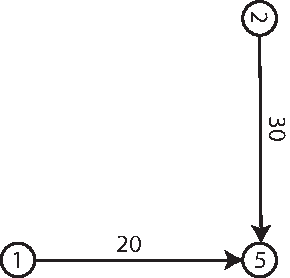
\includegraphics[scale=0.6]{fig/04model/05graphs}
		\subcaption{Traditional representation of the graph $(\{1,2,5\},\Set{30=(2,5),20=(1,5)})$.}
		\label{subfig:traditionalgraphtoNest}
	\end{minipage}\qquad \begin{minipage}{0.6\textwidth}
		\centering
		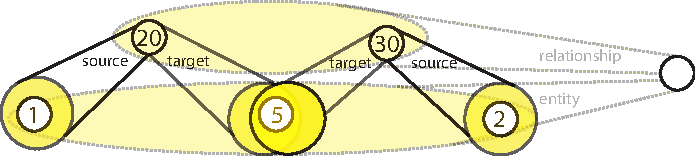
\includegraphics[scale=0.8]{fig/04model/05nested}
		\subcaption{Nested representation reflecting the actual structure of the data model.}
		\label{subfig:nestedreprofgraph}
	\end{minipage}
	\caption{Nested graph representation (\subref{subfig:nestedreprofgraph}) of a traditional graph data structure extended with edge id (\subref{subfig:traditionalgraphtoNest}).}
	\label{subfig:representableGraphs}
\end{figure}
\section{Nested Graph}\label{def:ngraph}
Despite the definition of efficient graph distributed models using a nested relational representation \cite{Labouseur2015}, a proper graph data model embodying a nested representation of graphs is missing. As we already saw, GSM allows to perform arbitrary nestings up to user-defined model constraints. Now, we must specialise this data model to distinguish the objects representing vertices from the ones representing edges; moreover, we want also that objects representing atoms should be distinguishable from the other two. The reason for doing this is that different kind of operations can be performed simultaneously over vertices and edges, as presented by the join operator in the last chapter. Therefore, instead of representing vertices and edges as belonging to the same set and then extract them in order to perform a distinct set of operations, we will directly distinguish the vertices and edges as belonging to two distinct properties of the same (reference) object.

\begin{definition}[Nested Graph]
	A \textbf{nested graph}\index{graph!nested graph} is a nesting loop free GSM $\fullnested$  where $\ngraph$ is an object containing both the vertex ($\phi(\ngraph,\ONTA)$) and edge ($\phi(\ngraph,\RELA)$) set. Each object $g\in \varphi^*(\ngraph)$ such that $\RELA\in\dom(\phi(g))\wedge \ONTA\in\dom(\phi(g))$ is said to be a \textbf{graph}. Each graph must satisfy the following properties:
	\begin{itemize}
		\item Each vertex $v'$ in $\ngraph$ is associated to a \ONTA collection ($\exists g\in\varphi^*(\ngraph). v'\in\phi(\ngraph,\ONTA)$).
		\item Each edge $e'$ in $\ngraph$ is associated to a \RELA collection ($\exists g\in\varphi^*(\ngraph).e'\in\phi(g,\RELA)$).
		\item  The same object shall not belong to both \ONTA or \RELA collections of any object\footnote{Please note that, by enforcing the model with such constraint, no RDF graph representation will be possible. On the other hand, alignment over the edges' types would not be formulated. As we will see on the later sections, we will not strictly perform such alignments at the nested graph level, but we will use general $GSM$ to do so. Nevertheless, the thesis will focus only on this nested graph model.} ($\bigcup_{o\in \varphi^*(\ngraph)}\phi(o,\ONTA)\;\cap\; \bigcup_{o\in \varphi^*(\ngraph)}\phi(o,\RELA)=\emptyset$).
		\item All the edge elements $e'$ must contain only two vertices $s$ and $t$ such that $s$ is a source for $e'$ ($\phi(e',\SRC)=[s]$) and $t$ is its target\footnote{More formally, $\forall o\in O.\forall e'\in\phi(o,\RELA).|\phi(e',\SRC)|=1\wedge |\phi(e',\DST)|=1$. Please note that, by relaxing such constraint to an arbitrary non-zero number of elements (that is, $s\in\phi(e',\SRC)$ with $|\phi(e',\SRC|\geq 1$ and $t\in\phi(e',\DST)$ with $|\phi(e',\DST)|\geq 1$), this representation allows to represent hypergraphs, that are graph representations where edges allow more than one possible source and edge.} ($\phi(e',\DST)=[t]$). Moreover, $s$ and $t$ must both be vertices ($\exists g,g'\in\varphi^*(\ngraph). s\in\phi(g,\ONTA)\wedge t\in\phi(g',\ONTA)$) Such elements are uniquely identified by a $\lambda$ function which is defined as follows:
		\[\lambda(o)\eqdef \phi(o,\SRC)\times\phi(o,\DST)\]
\end{itemize}
Given that are not specific on what a `graph' should be, both vertices and edges may represent (nested) graphs.
\end{definition}


\begin{figure}
	\centering
	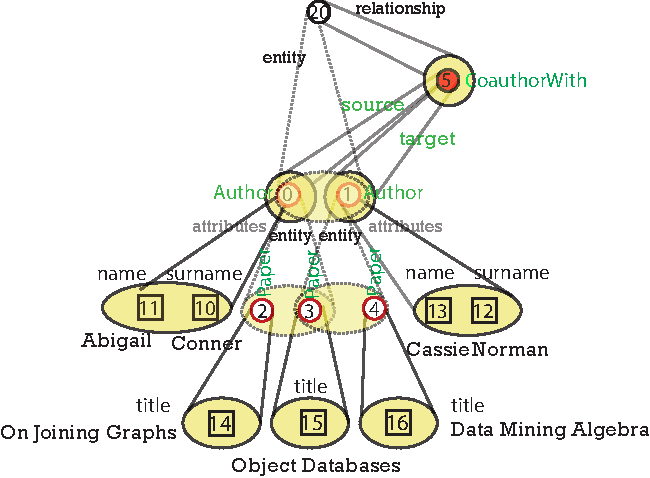
\includegraphics[width=\textwidth]{fig/04model/0405Full}
	\caption{Representation of a nested graph in different steps. This data structure represents ``Author Abigail Conner is Coauthor with Cassie Norman because they both authored the Paper ``Object Databases''. Abigail Conner also wrote ``On Joining Graphs'', while Cassie Norman wrote ``Data Mining Algebra''. From now on we will represent the objects with empty containments as squares, and the non-empty ones as circles. Edges are represented by circles filled in red, while vertices are represented by red bordered circles. Moreover, labels are placed above the nodes, while the expressions are placed below.}
	\label{fig:0405full}
\end{figure}

\begin{figure}
	\centering
	\hspace*{-2cm}
	\begin{minipage}{.5\textwidth}
		\centering
		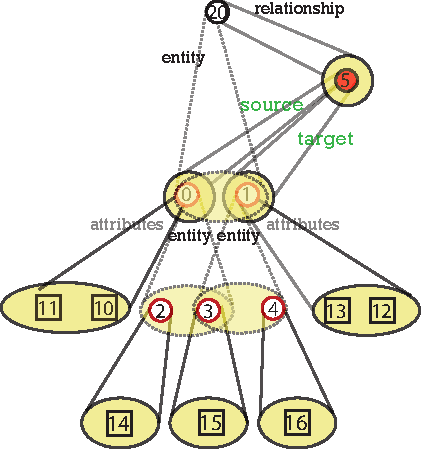
\includegraphics{fig/04model/0401Expressions_F}
		\subcaption{Expressions in $\xi$ for vertices and edges. \texttt{Entity}, \texttt{Relationship} and the edges' source and target information.}
		\label{fig:0402Labels}
	\end{minipage}\quad  \begin{minipage}{.5\textwidth}
	\centering
	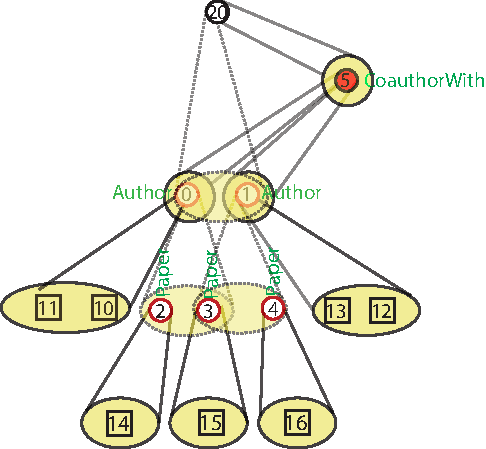
\includegraphics{fig/04model/0401Labels_F}
	\subcaption{Labels in $\ell$ for vertices and edges. Labels do only represent the objects' associated types.}
	\label{fig:0403Expressions}
\end{minipage} 
\medskip
\centering
\begin{minipage}{.8\textwidth}
	\centering
	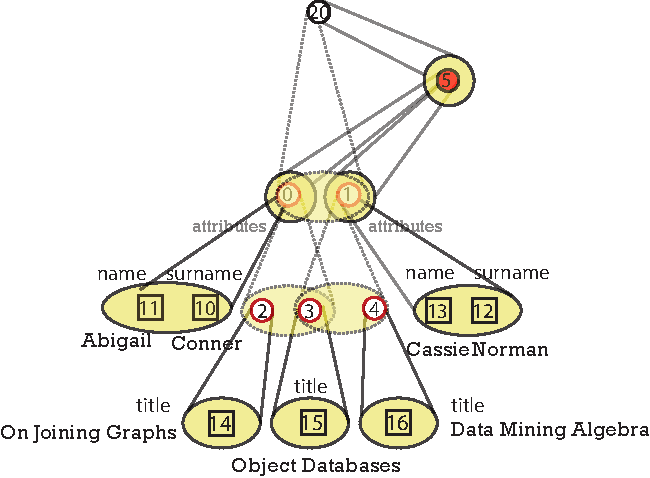
\includegraphics{fig/04model/0404Attributes_1}
	\subcaption{Labels and expressions for the attributes, that are objects containing neither \texttt{``Entity''} nor \texttt{``Relationship''} expressions. Their keys are expressed in $\ell$ while their values are stored as $\xi$ expressions.}
	\label{fig:0404Attributes}
\end{minipage}\quad 
	\caption{Analysing each component in Figure \vref{fig:0405full}. }
	\label{fig:nestingexample}
\end{figure}
The proposed nested graph data model provides a ``(nested) relational representation'' of a graph: vertices and edges are both represented as objects, and edges' source and target vertices are represented as edges' fields. Our model allows to nest (sub)graphs for each vertex and edge: this is due to the fact that an object can contain \mstr{Entity} and \mstr{Relationship} properties. Consequently, this data structure allows to represent traditional graphs and multigraphs, as outlined in Figure \vref{subfig:representableGraphs}. The actual trasformation function allowing to transform a graph into a nested graph representation will be provided in Section \vref{sec:tautonesting}, alongside with other data transformation representations.
The example that follows provide some insights on how such data structures can be used to represent nested components.

\begin{example}
Figure 6.3 provides a graphical representation of a nested graph.
\[N=(20,\Set{0,1,\dots,4,10,\dots,16,20},\ell,\lambda,\xi,\phi)\]
As we can see, the vertex set is $\phi(20,\ONTA)$ while the edge set is $\phi(30,\RELA)$. Consequently, those sets are represented as objects providing the following collections (i.e., lists):
\[\phi(20,\ONTA)=[0,1]\qquad \phi(20,\RELA)=[5]\]
Given that both vertices and edges are represented as objects, vertices and edges can contain other vertices and edges, too. Moreover, those objects can contain other objects, too, such as attributes, or the information of the edges' source and target vertices. In particular, such nested graph contains two authors, $0$ and $1$, which are coauthors. 
In particular, the coauthorship relation is represented by the edge $5$, which contains source and target elements as nested nodes:
\[\ell(0)=[\texttt{Author}]=\ell(1)\qquad \ell(5)=[\texttt{CoAuthorship}]\]
\[\phi(5,\SRC)=[0]\qquad \phi(5,\DST)=[1]\]
%\[\phi(30)=[5]\qquad \phi(5)=[0,1]\qquad  \ell(5)=[\texttt{CoAuthorship}]\qquad \xi(5)=[\texttt{``Relationship''}]\]
Moreover, each vertex nests the information of the papers that have been published by the containing author. Among this information, their names and surnames are also contained:
\[ \ell(2)=\ell(3)=\ell(4)=[\texttt{Paper}]\]
\[\phi(0,\ONTA)=[2,3]\quad \phi(0,\ATTR)=[11,10]\]
\[\phi(1,\ONTA)=[3,4]\quad \phi(0,\ATTR)=[13,12]\]
\[\ell(11)=\ell(13)=[\texttt{Name}]\qquad \xi(11)=[\mstr{Abigail}]\quad \xi(13)=[\mstr{Cassie}]\]
\[\ell(10)=\ell(12)=[\texttt{Surname}]\quad \xi(10)=[\mstr{Conner}]\quad \xi(12)=[\mstr{Norman}]\]
For each paper, the title information is also provided through object containment:
\[\ell(14)=\ell(15)=\ell(16)=[\texttt{Title}]\]
\[\xi(14)=[\mstr{On Joining Graphs}]\quad \xi(15)=[\mstr{Object Databases}]\quad \xi(16)=[\mstr{Data Mining Algebra}]\]
\end{example}

Please note that this graphical representation is verbose, and does  clarify which object is a vertex and which element is an edge only by its containment into a graph object. We call \textbf{simple vertex} (\textbf{simple edge}) a vertex (edge) which is not a graph. A more interesting example of Nested Graphs is going to be provided by Example \vref{ex:partof}.



%
%\section{Nested Graphs [OLD]}\label{def:ngraph}
%Nested graphs overcome the problems of the aforementioned data representations: with this proposed data model, both vertices and edges are objects (see MOF at Definition \vref{def:mof}), that is multi-labelled associations between attribute and values. Similarly to our previous definition of property graphs in Definition \vref{def:pg}, we associate to each object $o\in D_O$ a disambiguation identifier $i\in \mathbb{N}$ so that $o_i$ appears only once and $f_\Re(o)\oplus i$ is an unique id, where $f_\Re$ is the Skolem functor (see page \pageref{skolem}) and $\oplus$ is the concatenation function over integers (see page \pageref{def:concatenation}). By extending the previous model, nested graphs' values must represent either constant values, or objects' collections (for both vertices and edges) or aggregations over such collections. Given that our data model shall not impose any schema- and implementation-specific constraints, it allows different vertices and edges to (partially) share their content with other vertices and edges. Before providing some further examples and explanations, I now provide the formal definition for such data model:
%
%\begin{definition}[Nested Graph]\label{def:NestedGraphModelThesis}
%	\index{nested graph|textbf}
%Given a set of object-id pair $D_O\times\mathbb{N}$ and a language $\mathcal{L}_{MM}$, a \textbf{nested graph} is defined as a tuple $(V,E,A,\Lambda,\ell,\lambda,\iota)$, where each vertex $v_i\in V$ and each edge $e_k\in E$ are objects $v_i,e_k\in D_O\times \mathbb{N}$, where $v$ and $e$ describe the data content and $i$ and $k$ are disambiguating indices in order to distinguish $v_i$ and $e_k$ from all the other instances $v$ and $e$. Objects $v$ and $e$ are defined as functions $o\colon A\to \mathcal{L}_{MM}\times \mathcal{P}(D_O)$, mapping each attribute $a\in A$ to  a pair $(\textbf{e},s)$. In particular, $\textbf{e}\in \mathcal{L}_{MM}$ is an expression in language $\mathcal{L}_{MM}$ (hereby, it can be even a constant value) and $s$ is a set of objects over which $e$ can be evaluated into an arbitrary value expressible in both $V\cup E$ and $\mathcal{L}_{MM}$.
%
%In particular, to each edge is associated a pair of vertices $\lambda(e_k)\in V^2$, such that the first element of the pair is the source vertex and the second one is the target, and vertex and edge set are disjoint sets.
%Last, each vertex and edge is associated to a set of labels $\ell(o_j)\in \mathcal{P}(\Lambda)$. Last, $\iota:V\cup E\mathbb{N}$ is the indexing function associating to each vertex and edge an unique id.
%\bigskip
%
%\textbf{Notation}: we'll use the notation $o_i(\alpha)$ as a shorthand for $o(\alpha)$ of a given object-id pair $o_i$. We'll also use $\texttt{key}(o_j)$ to define the key set over which $o$ is defined and, in particular, the two following functions are defined:
%\[\texttt{ex}(o_j,k)=\texttt{fst}(o_j(k))=\texttt{fst}(e,s)=e\]
%\[\texttt{ls}(o_j,k)=\texttt{snd}(o_j(k))=\texttt{snd}(e,s)=s\]
%Moreover, we denote as $\Braket{k\mapsto (e,s)}$ as the singleton object which is only defined on key $k$ an which value $\Braket{k\mapsto (e,s)}(k)=(e,s)$.
%\end{definition}
%
%
%
%
%
